%%%%%%%%%%%%%%%%%%%%%%%%%%%%%%%%%%%%%%%%%%%%%%%%%%%%%%%%%%%%%%%%%%%%%%%%%%%%%%%%
%Objetivo: Descrever a implementação de uma extensão para uma FGRM de modo a
%avaliar o impacto este tipo de melhoria pode causar neste tipo de ferramenta.
%Autores: Vagner Clementino <vagnercs@dcc.ufmg.br>
%		  Rodolfo Resende <rodolfo@dcc.ufmg.br>
%Criação: dom fev 26 12:49:27 BRT 2017
%Modificação: qui mar  9 20:55:46 BRT 2017
%Revisão: dom mar 12 09:35:34 BRT 2017
%%%%%%%%%%%%%%%%%%%%%%%%%%%%%%%%%%%%%%%%%%%%%%%%%%%%%%%%%%%%%%%%%%%%%%%%%%%%%%%%
\chapter{Um Estudo sobre a Implementação de uma Extensão para FGRM}
\label{ch:implemtacao_extensao}

\section{Introdução}
\label{sec:implemtacao_extensao_intro}

Durante esta dissertação estamos discutindo que as funcionalidades oferecidas
pelas Ferramentas de Gerenciamento de Requisições de Mudança \@-\@ FGRMs
conseguem atender aos objetivos deste tipo de software. Todavia, verificamos que
exite espaço para melhorias das funções já existentes ou mesmo a proposição de
novas. O desenvolvimento de novas funcionalidades em FGRMs, mediante a
capacidade de extensão propiciada por algumas delas, vem sendo explorada na
literatura. A extensão
\textit{Buglocalizer}~\cite{Thung:2014:BIT:2635868.2661678}, criada para a
ferramenta Bugzilla, possibilita a localização dos arquivos do código fonte que
estão relacionados ao defeito relatado. A ferramenta extrai texto dos campos de
sumário e descrição da RM\@. Este texto é comparado com o código fonte por meio
de técnicas de Recuperação da Informação.

Na mesma linha, o \textit{NextBug}~\cite{101186} é uma extensão para o Bugzilla
que recomenda novas RMs para o desenvolvedor baseado naquela em que ele esteja
tratando atualmente. O objetivo da extensão é sugerir defeitos com base em
técnicas de Recuperação de Informação. Na ferramenta proposta por Thung e
outros~\cite{Thung:2014:DIT:2642937.2648627} o foco é na determinação de
defeitos duplicados. A contribuição deste trabalho é a integração do estado da
arte de técnicas não supervisionadas para detecção de falhas duplicadas conforme
proposto por Runeson e outros.

Esta dissertação também se propôs em contribuir com a melhoria das
funcionalidades das FGRMs mediante a apresentação e discussão de um conjunto de
recomendações conforme descrito no Capitulo~\ref{ch:sug_melhoria}. Apesar de ter
sido conduzido um processo de avaliação daquilo que foi proposto, cujo resultado
demonstrou uma boa aceitação dos participantes, optamos por analisar o impacto
da implementação do que foi proposto em determinada FGRM\@.

Conforme discutido, a Seção~\ref{sec:sug_melhoria_melhorando_as_ferraementas}
apresenta um conjunto de $N$ sugestões de melhorias das funcionalidades.
Idealmente gostaríamos de transformar todas as sugestões em extensões de
funcionalidades para as FGRMs. Não há razões que justifiquem a priorização de
implementação de uma recomendação sobre outra. Entretanto, após alguns ensaios e
combinando de maneira mais intuitiva do que seguindo um fluxo de critérios,  foi
investido mais esforço no desenvolvimento de uma extensão para o suporte à
qualidade de relato.

\section{Qualidade do Relato de uma RM}
\label{sec:avaliando_a_qualidade_do_relato_de_uma_rm}

No estudo realizado por Bettenburg e outros~\cite{bettenburg2008makes} foi
desenvolvida um levantamento com questionário (\textit{survey}) entre
desenvolvedores e usuários dos projetos
Apache\footnote{\url{http://www.apache.org/}},
Eclipse\footnote{\url{https://www.eclipse.org}} e
Mozilla\footnote{\url{https://www.mozilla.org}} a fim de verificar o que
produziria um bom relato de um RM\@. Os resultados demonstraram que do ponto de
vista dos desenvolvedores eram consideradas informações úteis, que idealmente
deveriam estar no relato de uma RM\@: \textit{(i)} a sequência de erros
executadas até o aparecimento do erro (se for o caso), também conhecida como
\textit{etapas para reproduzir}; \textit{(ii)} o registro de pilhas de ativação
(stack traces) que são arquivos com os histórico de chamada de métodos (logs)
que ocorreram antes da ocorrência do erro.

No estudo proposto por Zimmermann e outros~\cite{5070993} é discutido a
importância de que a informação descrita em uma RM seja relevante e completa a
fim de que esteja relatado seja resolvido rapidamente. Contudo, na prática, a
informação apenas chega ao desenvolvedor com a qualidade requerida após diversas
interações com o usuário afetado. Com o objetivo de minimizar este problema os
autores propõe um conjunto de diretrizes para a construção de uma extensão capaz
de reunir informações relevantes a partir do usuário além de identificar
arquivos que precisam ser corrigidos para resolver o defeito.

\section{Uma Extensão para Suporte da Qualidade do Relato}
\label{sec:uma_extensao_suporte_qualidade_relato}

\begin{description}
	\item[Questão 01:] Qual impacto da inclusão de uma extensão para o suporte à
		qualidade do relato pode ter no tempo necessário para análise de uma
		RM\@?
	\item[Questão 02:] Existe relação entre a frequência que um participante
		cria uma RM e a qualidade do relato?
	\item[Questão 03:] Do ponto de vista dos profissionais envolvidos em
		manutenção de software qual o impacto da inclusão de uma extensão para o
		suporte à qualidade do relato no processo de manutenção de software?
\end{description}

Na \textit{Questão 01} estamos interessados em verificar se a inclusão de uma
extensão deste tipo pode atrasar o processo de resolução de uma RM por conta da
eventual sobrecarga que a análise da qualidade do relato pode causar. A
\textit{Questão 02} possui o foco em avaliar se aquelas pessoas que criam RM com
maior frequência em determinado projeto possuem uma qualidade do relato superior
daqueles que fazem isso eventualmente. Por fim, na \textit{Questão 03} queremos
entender os prós e contras que a implantação deste tipo de extensão pode
produzir no processo de manutenção de software tomando com base a opinião de
profissionais da área.

\subsection{Desenho da Extensão}
\label{sub:desenho_da_extensao}

O objetivo da extensão é analisar de maneira automatizada a qualidade do relato
de uma \textit{issue} em repositórios do GitHub. No contexto da extensão
proposta, o elemento correspondente ao conceito de uma RM foi mapeado para o
elemento \textit{issue} no âmbito da plataforma Github. Um Repositório é o
elemento mais básico do GitHub e contém os arquivos do projeto (incluindo
documentação) e armazena o histórico de revisões de cada
arquivo\footnote{\url{https://help.github.com/articles/github-glossary/}}. A
execução da extensão resulta em um conjunto de dicas para o responsável por
redigir a \textit{issue} com o intuito de melhorar a qualidade da informação
fornecida no relato, por esta razão recebeu o nome de \textit{IssueQuality}.

\subsubsection{Visão Geral}
\label{ssub:implementacao_extensao_visao_geral}

A extensão proposta pode ser vista como um cliente para API do
Github\footnote{\url{https://api.github.com/}} que possibilita analisar a
qualidade da informação fornecida no relato. Uma visão geral sobre o
funcionamento da \textit{IssueQuality} pode ser visualizada na
Figura~\ref{fig:diagrama_funcionamento_issuequality}. A partir de uma lista
pré-definida de repositórios (1) a extensão solicita, através da API do Github
(2), o conjunto de \textit{issues} que estão com a situação \textit{``aberta''}
(etapas 3 e 4). Para cada uma das \textit{issues} recebidas, a ferramenta cria
um comentário por meio da API (5) que é registrado e armazenado na base de dados
do Github (etapas 6 e 7). A partir do comentário gerado o próprio Github se
encarrega de notificar (8) o responsável por relatar a \textit{issue} (9). A
partir desta notificação espera-se que o responsável inclua a informação
solicitada mediante a criação de um novo comentário.

\begin{figure}[htpb]
    \centering
    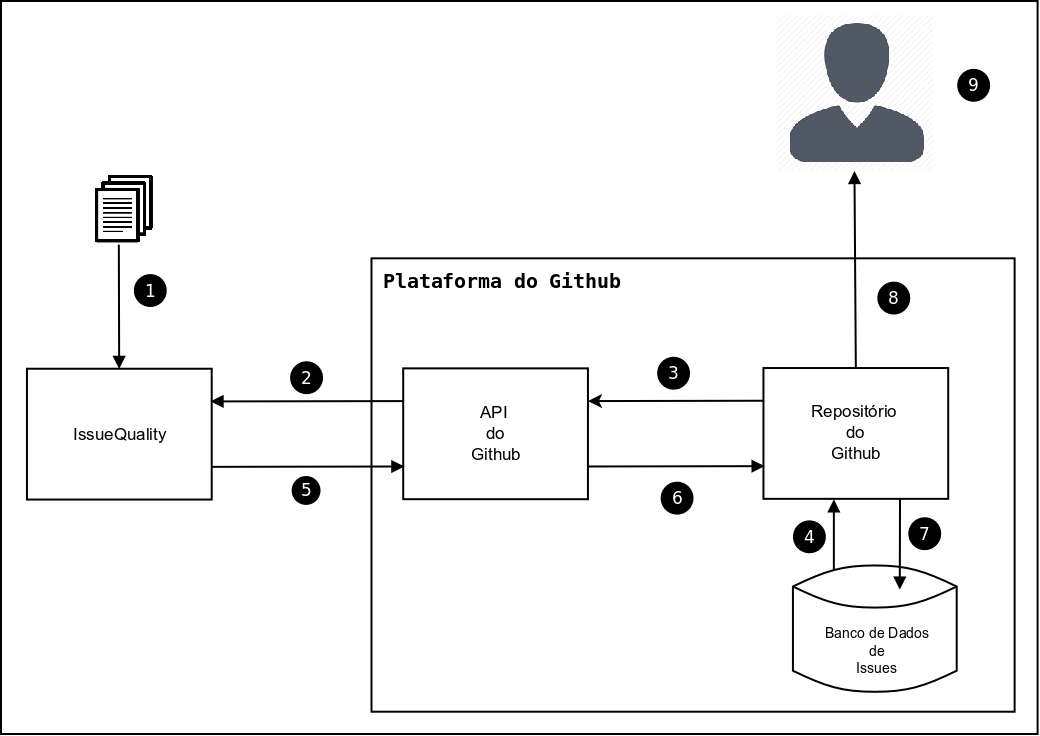
\includegraphics[width=0.7\linewidth]{chapter-implementacao-extensoes-fgrm/img/diagrama_funcionamento_issuequality.png}
    \caption{Visão geral do funcionamento da extensão \textit{IssueQuality}}
\label{fig:diagrama_funcionamento_issuequality}
\end{figure}

Para gerar o comentário descrito anteriormente, a extensão avalia alguns
atributos do texto que compõe o relato da RM\@. Os detalhes de como estes
atributos são analisados e o comentário é construídos estão descritos na próxima
seção.

\subsubsection{Análise da Qualidade do Relato}
\label{ssub:implementacao_extensao_analise_qualidade_do_relato}

Para cada issue analisada a extensão cria um \textit{vetor de características}
que armazena uma pontuação para cada atributo do texto que será analisado. Estes
valores podem ser binário (por exemplo, anexo presente ou não) ou contínuo (por
exemplo, legibilidade do texto). A análise dos atributos utilizam da sintaxe da
linguagem de marcação
Markdown\footnote{\url{https://help.github.com/categories/writing-on-github/}},
que é o padrão para as issues dos repositórios no GitHub.

Conforme descrito, o resultado da análise feita pela extensão é um comentário na
\textit{issue}. Em geral, ele é composto de três partes: \textit{cabeçalho,
    corpo e dicas}. O cabeçalho apresenta um texto padrão que é personalizado
com o nome do usuário (login) no Github do reportador. Ao utilizarmos a sintaxe
\textit{\@[Github loing]} o próprio Github se encarrega de enviar um e-mail
notificando o usuário sobre o comentário. A Figura~\ref{fig:issue_original}
exibe o cabeçalho padrão incluídos nos comentários.

\begin{figure}[htpb]
    \centering
    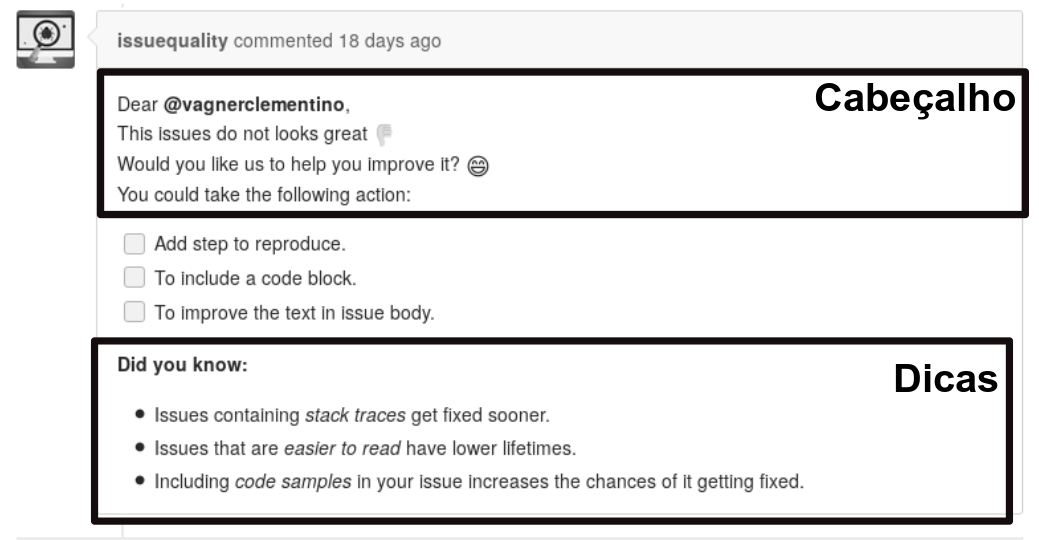
\includegraphics[width=0.8\linewidth]{chapter-implementacao-extensoes-fgrm/img/issue_original.png}
    \caption{Comentário produzido pela extensão IssueQuality com os cabeçalhos e
        dicas padrões.}
\label{fig:issue_original}
\end{figure}

Ao final do comentário é incluído um conjunto de dicas com objetivo de reforçar
com reportador os benefícios que a melhoria da qualidade do relato pode ter na
solução de sua \textit{issue}, como por exemplo dizendo que issues que são mais
fáceis de serem lidas possuem um tempo de solução menor. Estas dicas foram
obtidas com base na literatura sobre melhoria da qualidade do relato,
especialmente nos trabalhos de Bettenburg e outros~\cite{bettenburg2007quality,
    bettenburg2008makes}. Na Figura~\ref{fig:issue_original} é possível
visualizar como algumas dicas são apresentadas.

O corpo é parte mais dinâmica do comentário. Ele é construído incluindo
fragmentos de texto quando certos critérios de aceitação não foram atendidos.
Por exemplo, caso não seja detectado a presença de \textit{``etapas para
    reproduzir''} no relato de uma \textit{issue} o seguinte fragmento de texto é
incluído no corpo do comentário: \textit{``Add step to reproduce''}. Os
atributos avaliados e os critérios de aceitação estão descritos na
Tabela~\ref{tab:criterios_analise_qualidade_relato}.

\begin{table}[htpb]
\centering
\resizebox{\textwidth}{!}{%
\begin{tabular}{@{}cl@{}}
\toprule
\textbf{Atributo}             & \multicolumn{1}{c}{\textbf{Critério de Aceitação}}\\
\midrule
Completude de Palavras-Chaves & Existência de uma lista representando as etapa
executadas até ocorrência do erro.         \\
Arquivos Anexados             & Pelo menos um arquivo anexado a issue
\\
Fragmentos de Código          & Existência de pelo menos um fragmento de código
no relato da issue.                       \\
Completude do Texto           & As palavras que compõe o relato da issue devem
fazer parte de pelo menos duas categorias. \\
Legibilidade do Texto         & Dois testes de legibilidade apresentarem valores
acima dos limiares.                      \\ \bottomrule
\end{tabular}%
}
\caption{Critérios de aceitação e forma de análise utilizados na análise de
    qualidade do relato.}
\label{tab:criterios_analise_qualidade_relato}
\end{table}

O corpo do comentário é produzido com análise dos seguintes atributos do relato
da RM\@: \textit{Etapas para Reproduzir, Arquivos Anexados, Fragmentos de
    Código, Completude do Texto e Legibilidade do Texto}. Estes atributos foram
baseados no estudo realizado por Bettenburg e outros~\cite{bettenburg2008makes}.
A seguir apresentamos os detalhes como cada atributo é avaliado.

\paragraph{Etapas para Reproduzir:}
\label{par:etapas_para_reproduzir_}

Verifica se reportador incluiu uma lista, na forma de itens, descrevendo as
etapas executadas até a ocorrência da falha. Para detectar este padrão a
extensão aproveita da linguagem Markdown, que é o padrão utilizado para redigir
o relato da \textit{issue}, e que possui uma sintaxe pré-definida para listas. O
padrão é detectado através da utilização de expressões regulares. Pode ocorrer
que o Reportador utilize outro formato para relatar as etapas executadas até a
ocorrência da falha, contudo, o fato a extensão exigir a informação através de
uma lista, pode criar no Reportador uma boa prática. Cabe ressaltar que uma
lista com etapas para reproduzir foi uma das informações mais relevantes a
estarem no relato de uma RM~\cite{bettenburg2008makes}.

\paragraph{Arquivos Anexados:}
\label{par:arquivos_anexados}

Nesta dimensão avaliamos a existência de arquivos anexados à \textit{issue},
tais como capturas de telas (screenshots) e cadeia de registros de ativação de
funções (stact trace). A detecção é realizada utilização expressões regulares
utilizando da sintaxe padrão que é utilizada no relato da
RM\footnote{\url{https://guides.github.com/features/mastering-markdown/}}. Não
houve avaliação sobre o conteúdo do anexo, contudo, conforme descrito na
Tabela~\ref{tab:criterios_analise_qualidade_relato}, uma mensagem é incluída no
corpo do comentário no caso de nenhum anexo for detectado. A existência de
anexos em uma RM consta como uma das informações mais relevante do ponto de
vistas dos desenvolvedores~\cite{bettenburg2008makes}.

\paragraph{Fragmentos de Código}
\label{par:fragmentos_de_código}

Este atributo de avaliação verifica se fragmentos de código foi adicionado no
relato da \textit{issue}. O processo de detecção utilização de expressão
regulares e da sintaxe oferecida pela versão do Markdown utilizado pelo
Github\footnote{\url{https://guides.github.com/features/mastering-markdown/\#GitHub-flavored-markdown}}.
De forma similar aos atributos descritos anteriormente, a verificação de
fragmentos de código fonte é binária, ou seja, foi avaliada a existência ou não
de trecho de código.

\paragraph{Completude do Texto:}
\label{par:completude_de_palavras_chaves}

Nesta dimensão da avaliação há uma premissa que possa existir um vocabulário
comum no relato de diferentes RMs. Em outras palavras, algumas palavras aparecem
com determinada frequência no relato de uma RM, independente do projeto. Com o
objetivo de compreender como as pessoas descrevem problemas de software Ko e
outros~\cite{ko2006linguistic} analisar o título de 200.000 RMs de cinco
projetos de código aberto desenvolvidos na linguagem Java. Nos reutilizamos esta
base de dados\footnote{Disponível para download em
    \url{http://www.cs.cmu.edu/~marmalade/reports.html.}} para construir uma
distribuição da frequência de ocorrências de palavras no relato de uma RM\@.  Em
uma primeira etapa, removemos as palavras de parada (stopwords), reduzimos as
palavras\footnote{Do inglês \textit{stemming} é o processo de reduzir palavras
    flexionadas (ou às vezes derivadas) ao seu tronco (stem), base ou raiz,
    geralmente uma forma da palavra escrita. Por exemplo um algortimo de
    stemming reduz as palavras ``fishing'', ``fished'' e ``fisher'' para a raíz
    ``fish''.} e selecionamos as \textit{100} palavras com maior frequência. Em
seguida, categorizamos as palavras nos seguintes grupos:

\begin{itemize}

    \item itens de ação (do, work,open)
    \item relacionado com compilação (build, task)
    \item relacionado com documentação (support, help, content)
    \item comportamento esperado ou observável (fail, error, crash)
    \item relacionado com projeto (management, list)
    \item relacionado com código fontesource code-related (java, code, method)
    \item elementos da interface do usuário (menu, display, button)

\end{itemize}

\paragraph{Legibilidade do Texto}
\label{par:legibilidade_do_texto}

Por fim a extensão avalia o nível legibilidade do texto com base em testes
largamente utilizados na literatura~\cite{Si:2001:SMS:502585.502695}. Os testes
de legibilidade são fórmulas para avaliar a legibilidade do texto, geralmente
contando sílabas, palavras e frases.  Neste estudo utilizamos os testes de
legibilidade \textit{Flesch–Kincaid, Automated Readability Index \@-\@ ARI e
    Dale–Chall Readability Formula}. Os testes foram selecionados por
apresentarem metodologias distintas para determinar a legibilidade do texto.

O Flesch-Kincaid (FK) é baseado no número de sílabas das palavras que compõem as
sentenças do texto. Existem dois testes, o Flesch Reading Ease e Flesch–Kincaid
Grade Level, que diferem pelo fator de ponderação utilizado. A extensão utilizou
o Flesch Reading Ease que recebe um texto em língua inglesa e retorna um valor
inteiro representando a dificuldade de entendimento. Pontuações mais altas
indicam que o material é mais fácil de ler~\cite{kincaid1975derivation}. Desta
forma, foi considerada como legibilidade baixa uma pontuação \textit{menor do
    50}. Este valor foi baseado em uma tabela pré-definida pelo próprio
teste~\cite{kincaid1975derivation}.

O ARI considera o número de caracteres de cada palavra. O resultado do teste é
uma representação aproximada do grau de escolaridade americano necessário para
compreender o texto~\cite{senter1967automated}. De maneira aproximada, o grau 1
corresponde a idades 6\@-\@8. O nível de leitura 8 corresponde a jovem de 14
anos. O grau 12, o mais alto no ensino secundário dos EUA, corresponde ao nível
de leitura de 17 anos de idade.

Por outro lado, o teste Dale-Chall é baseado em um conjunto mínimo de palavras.
A fórmula usa uma lista de 3000 palavras que grupos de estudantes americanos de
quarta série poderiam entender de forma confiável, partindo-se da premissa que
qualquer palavra nessa lista não seja de difícil~\cite{dale1948formula}. No caso
dos testes ARI e Dale-Chall a legibilidade será considerada ruim se o número de
anos de estudos necessário para o entendimento \textit{for maior ou igual a 13}
que representa de maneira geral e foi utilizado no trabalho de Bettenburg e
outros~\cite{bettenburg2008makes}.

\section{Avaliação da Extensão}
\label{sec:avaliando_a_extensao_proposta}

Com o objetivo de avaliar a extensão proposta conduzimos um levantamento
(survey) através questionário com profissionais que contribuem em projeto de
código aberto hospedados no Github. A metodologia utilizada na condução do
levantamento é descrita na próxima subseção.

\subsection{Desenho da Avaliação}
\label{sub:implementacao_extenscao_desenho_da_avaliacao}

Para realizarmos a coleta dos dados foi utilizado um levantamento (survey)
através de um questionário eletrônico. O processo de seleção dos participantes,
o desenho do questionário e como foi realização a sua aplicação estão descritos
na próximas subseções.

\subsubsection{Seleção dos Participantes}
\label{ssub:sug_melhoria_selecao_participantes}

Ficou definido que o público-alvo deste questionário seria profissionais que
façam uso de FGRMs e que desta forma possam obter as vantagens da extensão
propostas. Como este perfil é bastante genérico, optamos por utilizar uma
amostra de conveniência através de que atuam como \textit{contribuidores} em três
projetos de código aberto hospedados no Github. Dentre os contribuidores de um
projeto não houve nenhum critério de seleção, neste sentido todos poderiam
eventualmente participar da pesquisa. Os seguintes critérios foram
definidos para a escolha de um projeto:

\begin{itemize}
	\item Os projetos deve ser escrito prioritariamente em Java.
    \item Os projetos devem ter no mínimo 100 issues registradas.
	\item Os projetos devem ter no mínimo seis meses de desenvolvimento, para
		evitar projetos que não tenham passado por um tempo de manutenção
		relevante.
	\item Os projetos devem  ter  no  mínimo  200  revisões (commits)  pelos
		mesmos motivos  da restrição anterior.
	\item Os projetos escolhidos não devem ser ramificações (\textsl{branches}) um
		do outro projeto, para evitar dados duplicados.
	\item Os projetos obtidos devem ser os 10 mais populares que atendem aos
		demais critérios, utilizando como métrica o campo \texttt{most stars}
\end{itemize}

Após aplicação dos critérios descritos obtivemos os projetos descritos na
Tabela~\ref{tab:projetos_utilizados}. Conforme pode ser observado os projetos
selecionados referem-se a ferramentas bem estabelecidas e largamente utilizadas
por organizações e projetos de código aberto.

\begin{table}[htpb]
\centering
\resizebox{\textwidth}{!}{%
\begin{tabular}{@{}lccccc@{}}
\toprule
\multicolumn{1}{c}{\textbf{Projeto}} & \textbf{Revisões} & \textbf{Ramificações}
& \textbf{Lançamentos} & \textbf{Contribuidores} &
\textbf{Contrib\. com E-mail} \\ \midrule
elasticsearch & 27.118 & 94 & 174 & 812 &  \\
guava & 4.081 & 84 & 175 & 103 &  \\
spring-framework & 14575 & 12 & 106 & 211 &  \\ \bottomrule
\end{tabular}%
}
\caption{Projetos utilizados no levantamento com profissionais. Os dados
	apresentados tem como referência 23/04/2017.}
\label{tab:projetos_utilizados}
\end{table}

Com base nos projetos selecionados ficou definido que a amostra a ser utilizada
no levantamento seria os respectivos contribuidores. Um contribuidor é alguém
que participa efetivamente do desenvolvimento de um projeto, tendo o privilégio
de acesso para alterar o código fonte. O contato com os contribuidores foi
realizado por correio eletrônico, todavia, conforme pode ser verificado na
coluna \textit{Contrib.\ com E-mail} nem todos permitem acesso público ao seu
endereço.

\subsubsection{Desenho do Questionário}
\label{ssub:sug_melhoria_desenho_questionario}

Para avaliarmos a extensão desenvolvemos um questionário composto de duas
partes. Na primeira o objetivo é que participante emita opinião sobre a
qualidade do relato de uma issue do projeto que contribui bem como do grau de
relevância do comentado gerado pela extensão. Com este objetivo no desenhamos um
processo de avaliação conforme descrito a seguir. A descrição toma com base um
único projeto, contudo, a mesma metodologia foi replicada para os demais.

Nós selecionamento uma amostra aleatória de 50 \textit{issues} do projeto que
foram apresentados uma por uma aos participantes em uma ordem aleatória. Eles
eram obrigados a visualizar o relato da \textit{issue} e classificá-lo em uma
escala Likert de cinco pontos variando de muito ruim (1) a muito bom (5). Logo
em seguida era apresentado o comentário gerado pela extensão que precisa ser
classificado através de uma escala de cinco ponto que variava de Nada Relevante
até Muito Relevante. Também foi disponibilizado um campo de texto de
preenchimento facultativo do qual o participante poderia incluir informações
adicionais.

Uma vez que o participante classificou o relato da \textit{issue} e o comentário
gerado o formulário exibe uma nova \textit{issue} de forma aleatória. Os
desenvolvedores poderiam interromper a avaliação a qualquer momento ou optar por
continuar até que todos as 50 \textit{issues} do seu projeto tenham sido
classificadas.

A segunda parte é composta por questões sobre a formação de base (background) do
participante. Este conjunto de perguntas não eram de preenchimento obrigatório.
A Figura~\ref{} exibe uma parte do formulário utilizado neste estudo.

\todobegin{Incluir figura com o formulário}

\subsubsection{Processo de Aplicação}
\label{ssub:processo_de_aplicação}

O questionário foi encaminhado à amostra de interesse através de correio
eletrônico. O endereço foi coletado diretamente do projeto hospedado no Github.
Foi desenvolvido um \textit{script} na linguagem Python que permitia coletar o
endereço de e-mail e automatizar o processo de envio. As mensagem foram
personalizadas de modo a identificar o nome do usuário e o projeto do Github com
base no template exibido a seguir.

\todobegin{Incluir o quadro com o template de envio das mensagens.}

\subsection{Resultados}
\label{sub:implementacao_extensao_avaliacao_resultados}

\subsection{Discussão}
\label{sub:implemtacao_extensao_avaliacao_discussao}

\section{Limitações e Ameças à Validade}
\label{sec:limitações_e_ameças_à_validade}

\section{Conclusões}
\label{sec:conclusões}

\section{Resumo do Capítulo}
\label{sec:implemtacao_extensao_resumo}
